\documentclass[11pt]{article}
\usepackage[utf8]{inputenc}

% MATH
\usepackage{amssymb}
\usepackage{amsmath}
\usepackage{amsthm}
\usepackage{mathtools}

%\newtheorem{cusdef}{Def}
%\newtheorem{custhm}{Thm}
%\newtheorem{cuscor}{Cor}
%\newtheorem{cusrk}{Rk}
\newenvironment{cusenv}[2]
{\begin{samepage}\noindent\textbf{#1} -- (#2) \par}
{\end{samepage} \bigskip}

\newenvironment{cusdef}[1]
{\begin{cusenv}{Def}{#1}}{\end{cusenv}}

\newenvironment{custhm}[1]
{\begin{cusenv}{Thm}{#1}}{\end{cusenv}}

\newenvironment{cuscor}[1]
{\begin{cusenv}{Cor}{#1}}{\end{cusenv}}

\newenvironment{cusprop}[1]
{\begin{cusenv}{Prop}{#1}}{\end{cusenv}}

\newenvironment{cusrk}[1]
{\begin{cusenv}{Rk}{#1}}{\end{cusenv}}	

% MISE EN FORME
\usepackage[left=2cm,right=2cm,top=2cm,bottom=2cm]{geometry}
\usepackage{titlesec}
\titleformat{\section}
{\Large\bfseries\normalfont\scshape}{}{0em}{}
\titleformat{\subsection}
{\large\bfseries\normalfont\scshape}{}{0em}{}
\titleformat{\subsubsection}
{\bfseries\normalfont\scshape}{}{0em}{}

\usepackage{hyperref}
\usepackage{xcolor}
\hypersetup{
	colorlinks,
	linkcolor={red!50!black},
	citecolor={blue!50!black},
	urlcolor={blue!80!black}
}


% MACROS
\usepackage{xparse}
\newcommand{\smbox}[1]{\mbox{\footnotesize #1}}
\newcommand{\A}{\mathcal{A}}
\newcommand{\Am}{\mathbb{A}}
\newcommand{\N}{\mathbb{N}}
\newcommand{\C}{\mathbb{C}}
\renewcommand{\P}{\mathbb{P}}
\newcommand{\R}{\mathbb{R}}
\newcommand{\K}{\mathbb{K}}
\newcommand{\M}{\mathbb{M}}
\newcommand{\topo}{\mathcal{T}}
\newcommand{\Lin}{\mathcal{L}}
\newcommand{\Int}{\mbox{Int}\,}
\newcommand{\st}{~\mbox{s.t.}~}
\newcommand{\miff}{~\mbox{iff}~}
\newcommand{\ie}{\emph{i.e.} }
\newcommand{\ms}{~~~}
\newcommand{\norm}[1]{\left|\left|#1\right|\right|}
\newcommand{\dual}[1]{#1'}
\newcommand{\sca}[2]{\big<#1, #2\big>}
\newcommand{\cont}[1]{\mathcal{C}^{#1}}
\title{Rapport TP X01 \\ TP1}
\author{Aurélien Valade}
\date{}

\begin{document}
\maketitle

\section{Intruction et structure du code}


Le but de ce TP est de résoudre le problème suivant : trouver $u \in H^1_0(\Omega)$ tel que  
\begin{equation}
  \begin{cases}
    u - \nabla \big(A(x,y) \nabla u\big) = f \ms \mbox{sur}\ms \Omega\\
    u = 0 \ms \mbox{sur}\ms \partial\Omega.
  \end{cases}
\end{equation}

La structure du code ainsi que l'arrangement des dossiers ont été un peu modifiés. Tous les \texttt{*.msh} se trouvent dans le dossier \texttt{geoms/} avec un executable \texttt{bash} pour en créer à volonté.

De plus, le corps de la routine principale se trouve maintenant dans \texttt{principal\_neumann\_aux.m}, cependant le fichier script est toujours bien \texttt{principal\_neumann.m}. 

Un code de calcul formel rédigé en python a été ajouté. 

Dans la suite, les intégrale dont le domaine n'est pas précisé portent sur tout $\Omega$.
\section{Q1}

Soit $\forall v\in H^1_0(\Omega)$.

\begin{align}
  \label{eq:var}
  &\int_{\Omega} uv - \int_{\Omega} \nabla \big(A(x,y) \nabla u\big) v = \int_{\Omega} f v && IPP \\
  &\int_{\Omega} uv - \int_{\partial \Omega} \big(A(x,y) \nabla u\big) v + \int_{ \Omega} A(x,y) \nabla u \nabla v  = \int_{\Omega} f v  && CL\\
  &\int_{\Omega} uv + \int_{ \Omega} A(x,y) \nabla u \nabla v  = \int_{\Omega} f v \\
  &a(u,v) = l(v)
\end{align}

On a bien $a(u,v)$ et $l(v)$ (bi)linéaires. Montrons que $a(u,v)$ continue 
\begin{align}
  \label{eq:ac}
  |a(u,v)| &\leq \left| \int A \nabla u \nabla v \right| + \left| \int u v \right| && \mbox{ineg. triang} \\
           &\leq \beta \left| \int \nabla u \nabla v \right| + \left| \int u v \right| && \mbox{A bornée} \\
           &\leq \beta \norm{\nabla u}_{L^2} \norm{\nabla v}_{L^2} + \norm{u}_{L^2}\norm{v}_{L^2} && \mbox{Cauchy Schwarz} \\
           &\leq \beta \norm{\nabla u}_{H^1_0} \norm{\nabla v}_{H^1_0} + \norm{u}_{H^1_0}\norm{v}_{H^1_0} && \norm{\cdot}_{L^2}<\norm{\cdot}_{H^1_0} \\
           &\leq (\beta+1) \norm{\nabla u}_{H^1_0} \norm{\nabla v}_{H^1_0}   \\
\end{align}

On a évidement $l(v)$ continue comme $f, v \in H^1_0(\Omega)$. 

Montrons que $a(u,v)$ est coercive
\begin{align}
  \label{eq:co}
  |a(u,u)| &\geq \left|\int A (\nabla u)^2 \right| + \left|\int u^2 \right| \\
           &\geq \max(A) \left|\int (\nabla u)^2 \right| + \left|\int u^2 \right| \\
           &\geq \xi \left|\int (\nabla u)^2 \right| + \left|\int u^2 \right| \\
           &\geq \min(\xi,1) \norm{u}_{H^1_0}
\end{align}

\section{Q2}

On onsidère uniquement $V_h \subset H^1_0(\Omega)$ de dimension finie, donc entièrement décrit par sa base $(\omega_I)_{1\leq I \leq N}$. Le problème se ramène donc à
\begin{equation}
  a(u,\omega_I) = l(\omega_I) \ms \forall 1\leq I\leq N.
\end{equation}

Si on projète $u$ sur la base des $(\omega_I)$ :
\begin{equation}
  u_h = \sum_{1}^{N} u_h^I \omega_I
\end{equation}
on retrouve le problème variationel entièrement discrétisé :
\begin{equation}
  \sum_J u_h^J a(\omega_I, \omega_J) = l(\omega_I) \ms \forall  1\leq J\leq N.   
\end{equation}

En posant les matrices et les vecteurs:
\begin{align}
  &U \in \R^{N}, \ms U_{I} = u_h^I, \\
  &L \in \R^{N}, \ms L_{I} = \int f \omega_I, \\
  &\K \in \R^{N\times N},\ms \K_{IJ} = \int A \nabla \omega_I \nabla \omega_J,  \\
  &\M \in \R^{N\times N},\ms \M_{IJ} = \int \omega_I \omega_J,
\end{align}
on peut écrire le système sous forme matricielle :
\begin{equation}
  (\M+\K) U = L.
\end{equation}


\section{Q3-Q4-Q5-Q6} 

On peut se ramener à un problème de taille $N^0 = \mbox{dim}(V^0_h)$ en considérant la matrice
\begin{gather}
  \Am = \M + \K \in \R^{N\times N } \\
  \Am^0 \in \R^{N^0\times N^0} \\
  \P \in \R^{N^0\times N} \\
  \Am^0 = \P\Am\P^T, ~ L^0 = \P L, ~ U^0 = \P U 
\end{gather} 
On construit la matrice $\P$ de la manière suivante
\begin{equation}
  \P = Id_N \mbox{~privée des lignes $i<N$ telles que $Refneu(i)\neq 0$.}
\end{equation}
Une fois le système $\Am^0 U^0 = L^0$ inversé, on peut retrouver $U$ par la formule $U=\P^T U^0$.

\section{Q7}

En utilisant le code de calcul formel, on trouve que
\begin{equation}
  f(x,y) = (1+5\pi^2)\cos(\pi x)\cos(2\pi y) \ms \forall x,y\in\Omega.
\end{equation}

\section{Q8}



Pour toute fonction
\begin{align}
  u = \sum_I u\big(S(I)\big) \omega_I \\
  U = \big(u(S(I))\big)_I \in \R^{ N}
\end{align}
on a que
\begin{align}
  \norm{u}_{L^2}^2 &= \big<u, u\big> \\
                   &= \sum_I \sum_J U_I U_J \big< \omega_I, \omega_J\big> \\
                   &= \sum_I \sum_J U_I U_J \M_{IJ} \\
                   &= U^T \M U \geq 0 \ms \mbox{car $\M$ définie positive,}
\end{align}
et de même
\begin{align}
  \norm{u}_{\smbox{semi~} H^1_0}^2 &= \big|U^T \K U \big|.
\end{align}

On peut donc lancer le programme et calculer les erreurs normalisées
\begin{align}
  err_{L^2} &= \frac{\norm{u_h-\pi_h u}_{L^2}}{\norm{\pi_h u}_{L^2}} \\
  err_{\smbox{semi~} H^1_0} &= \frac{\norm{u_h-\pi_h u}_{\smbox{semi~}H^1_0}}{\norm{\pi_h u}_{\smbox{semi~}H^1_0}} 
\end{align}
tracées en \autoref{fig:acst}

Pour ce qui du calcul de la fonction $f(x,y)$, grace au code python de calcul formel, on peut trouver que pour
\begin{equation}
  A(x,y)= \sin(\alpha \pi x)\sin(\alpha \pi y) + 2
\end{equation}
et si on veut garder comme solution
\begin{equation}
  u(x,y)=\sin(\pi x)\sin(2\pi y)
\end{equation}
il faut poser
\begin{equation}
  \begin{aligned}[t]
    f(x,y) =~& 2 \pi^2 \alpha \sin(\pi x) \sin(\pi \alpha x) \cos(2 \pi y) \cos(\pi \alpha y) - \\
    &\pi^2 \alpha \sin(2 \pi y) \sin(\pi \alpha y) \cos(\pi x) \cos(\pi \alpha x) + \\
    &5 \pi^2 (\sin(\pi \alpha x) \sin(\pi \alpha y) + 2) \sin(\pi x) \sin(2 \pi y) + \\
    &\sin(\pi x) \sin(2 \pi y).
  \end{aligned}
\end{equation}


\begin{figure}
  \centering
  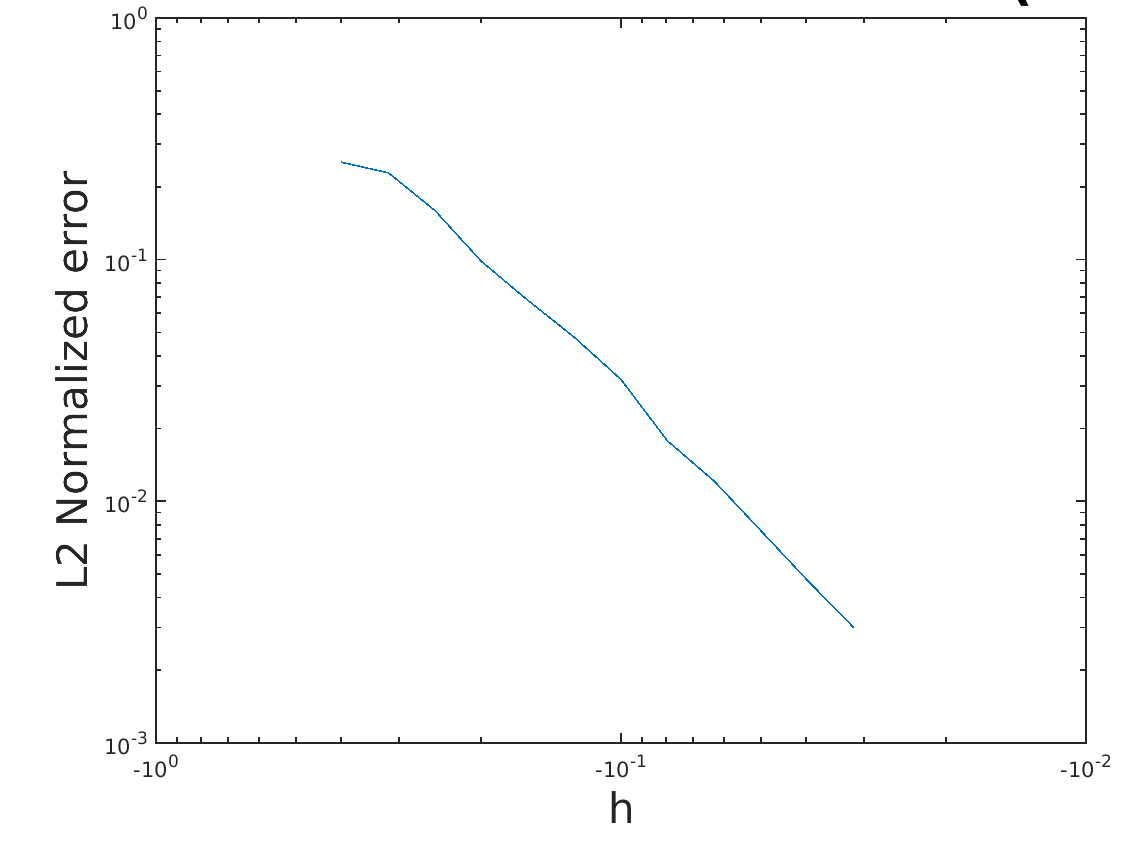
\includegraphics[width=.5\textwidth]{dirichlet/L2_Acst} 
  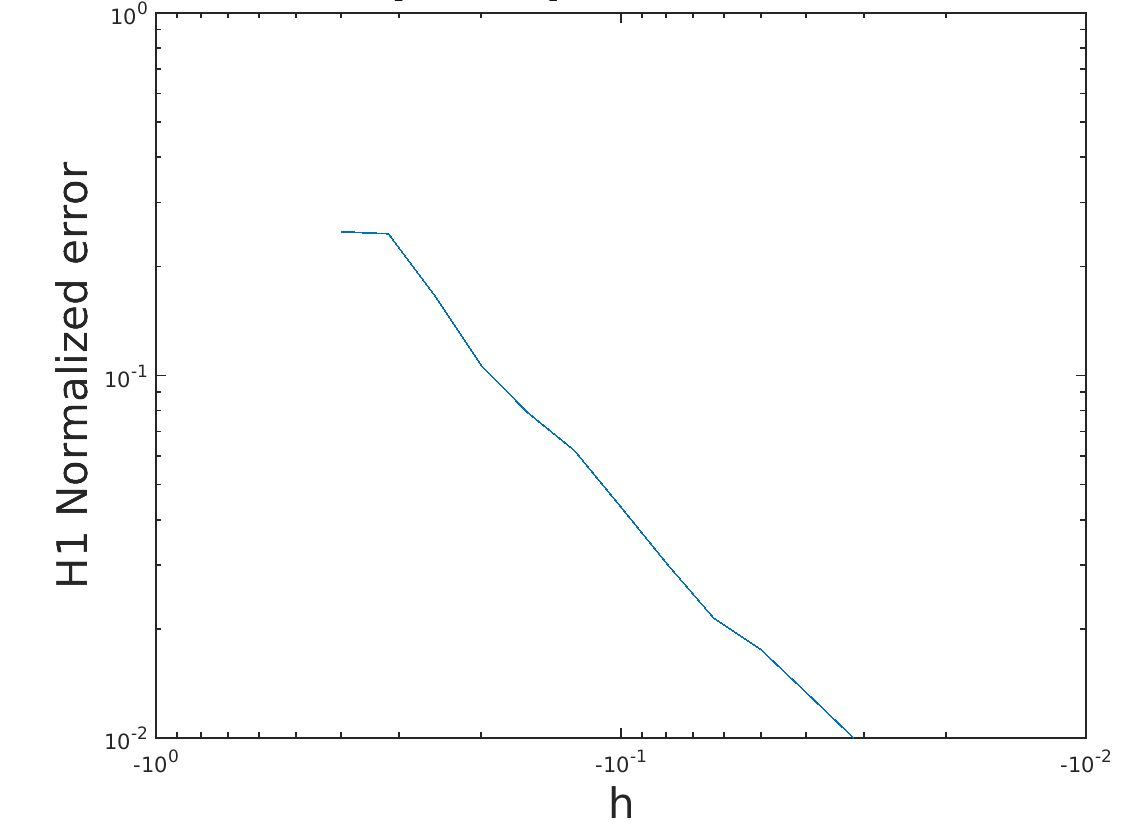
\includegraphics[width=.48\textwidth]{dirichlet/H1_Acst} \\
  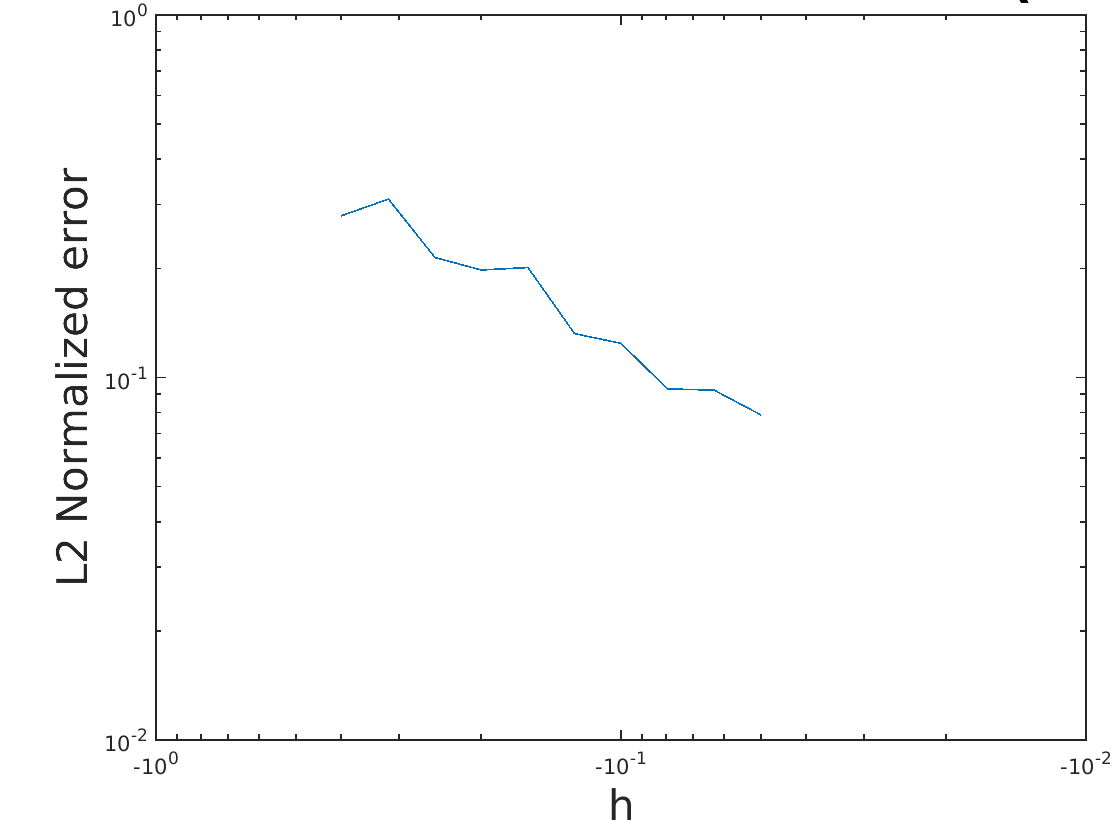
\includegraphics[width=.48\textwidth]{dirichlet/L2_Avar} 
  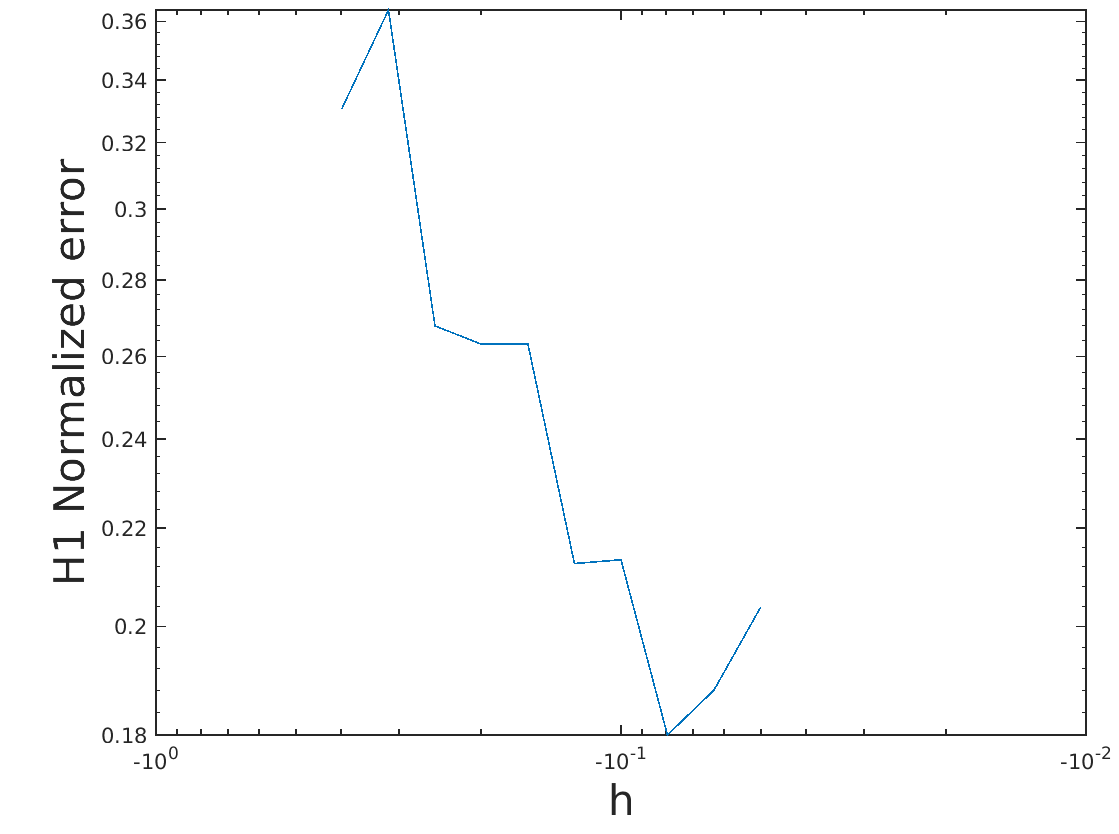
\includegraphics[width=.48\textwidth]{dirichlet/H1_Avar}
  \caption{Erreur normalisée pour la norme L2 et erreur normalisée pour la norme H1 dans le cas A constant.}
  \label{fig:acst}
\end{figure}

\section{Q8}

Montrons que le problème $a(u,v) = l(u) \ms \forall v \in V^h_{\#}$ est bien posé dans
\begin{equation}
  H^1_{\#}(\Omega) = \bigg\{ f \in H^1(\Omega), \mbox{tq $f$ est $L$ périodique} \bigg\}
\end{equation}
Montrons d'abord que $a$ est continue
\begin{align}
  \label{eq:ac}
  |a(u,v)| &\leq \left| \int A \nabla u \nabla v \right| + \left| \int u v \right| && \mbox{ineg. triang} \\
           &\leq \beta \left| \int \nabla u \nabla v \right| + \left| \int u v \right| && \mbox{A bornée} \\
           &\leq \beta \norm{\nabla u}_{L^2} \norm{\nabla v}_{L^2} + \norm{u}_{L^2}\norm{v}_{L^2} && \mbox{Cauchy Schwarz} \\
           &\leq \beta \norm{\nabla u}_{H^1_{\#}} \norm{\nabla v}_{H^1_{\#}} + \norm{u}_{H^1_{\#}}\norm{v}_{H^1_{\#}} && \norm{\cdot}_{L^2}<\norm{\cdot}_{H^1_{\#}} \\
           &\leq (\beta+1) \norm{\nabla u}_{H^1_{\#}} \norm{\nabla v}_{H^1_{\#}}   \\
\end{align}

On a évidement $l(v)$ continue comme $f, v \in H^1_{\#}(\Omega)$. 

Montrons que $a(u,v)$ est coercive
\begin{align}
  \label{eq:co}
  |a(u,u)| &\geq \left|\int A (\nabla u)^2 \right| + \left|\int u^2 \right| \\
           &\geq \max(A) \left|\int (\nabla u)^2 \right| + \left|\int u^2 \right| \\
           &\geq \xi \left|\int (\nabla u)^2 \right| + \left|\int  u^2 \right| \\
           &\geq \min(\xi,1) \norm{u}_{H^1_{\#}}
\end{align}

\section{Q9}

On peut se ramener à un problème dans $V^{\#}_h$ en considérant la matrice
\begin{gather}
  \Am = \M + \K \in \R^{N\times N } \\
  \P \in \R^{N\times N} \mbox{~inversible}\\
  \Am^{\#} = \P^{-1}\Am^{\#}\P, ~ L^{\#} = \P^{-1} L, ~ U^{\#} = \P^{-1} U 
\end{gather} 
On construit la matrice $\P$ de la manière suivante
\begin{equation}
  \forall I,J \in [1,N]^2 \ms
  \P_{IJ} =
  \begin{cases}
    4 \delta_{IJ} \ms \mbox{si~} S(I) \mbox{~est sur un angle} \\
    2 \delta_{IJ} \ms \mbox{si~} S(I) \mbox{~est sur un bord} \\
    \delta_{IJ} \ms \mbox{sinon}
  \end{cases}
\end{equation}
Une fois le système $\Am^0 U^0 = L^0$ inversé, on peut retrouver $U$ par la formule $U=\P^{-1} U^{\#}$.

\section{Q10}

Pour ce qui du calcul de la fonction $f(x,y)$, grace au code python de calcul formel, on peut trouver que pour
\begin{equation}
  A(x,y)= \sin(\alpha \pi x)\sin(\alpha \pi y) + 2
\end{equation}
et si on veut garder comme solution
\begin{equation}
  u(x,y)=\cos(\pi x)\cos(2\pi y)
\end{equation}
il faut poser
\begin{equation}
  \begin{aligned}[t]
    f(x,y) =~& \pi^2 \alpha \sin(\pi x)  \sin(\pi \alpha y)  \cos(2 \pi y)  \cos(\pi \alpha x) - \\
          &2 \pi^2 \alpha \sin(2 \pi y)  \sin(\pi \alpha x)  \cos(\pi x)  \cos(\pi \alpha y) + \\
          &5 \pi^2 (\sin(\pi \alpha x)  \sin(\pi \alpha y) + 2)  \cos(\pi x)  \cos(2 \pi y) + \\
          &\cos(\pi x)  \cos(2 \pi y).
  \end{aligned}
\end{equation}

\begin{figure}
  \centering
  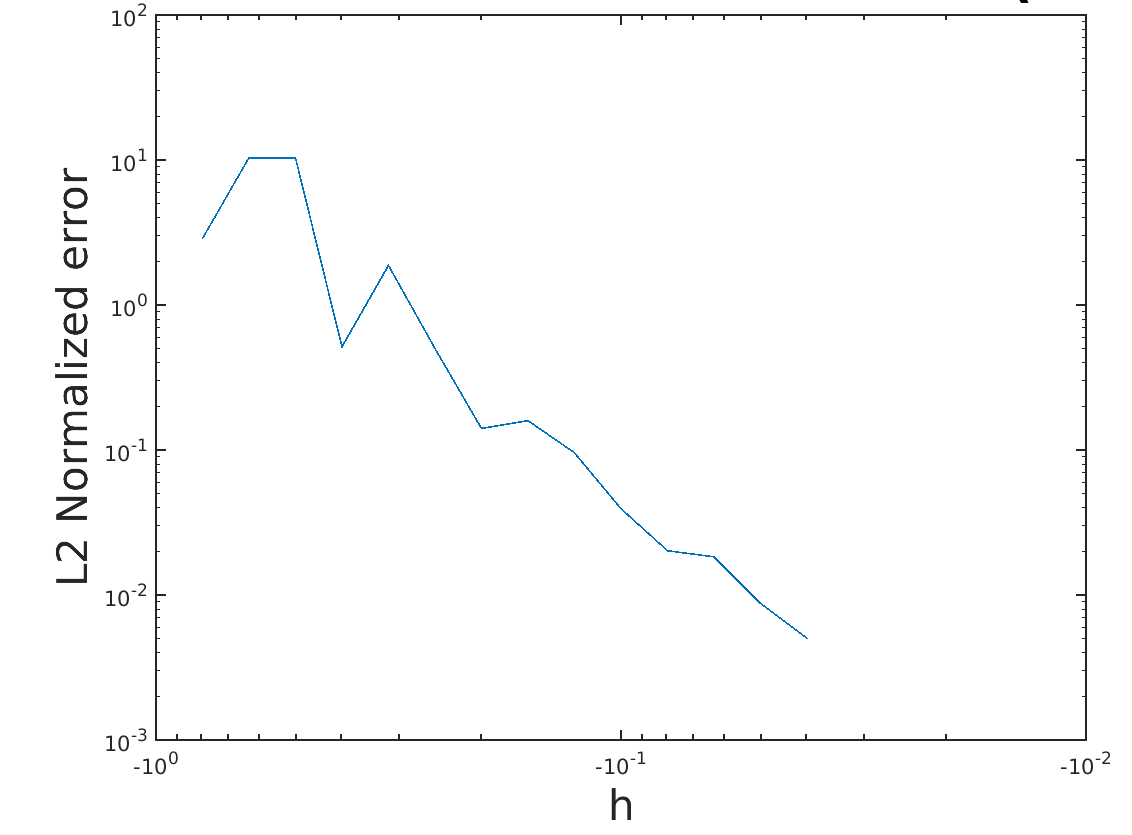
\includegraphics[width=.48\textwidth]{periodique/L2_Acst} 
  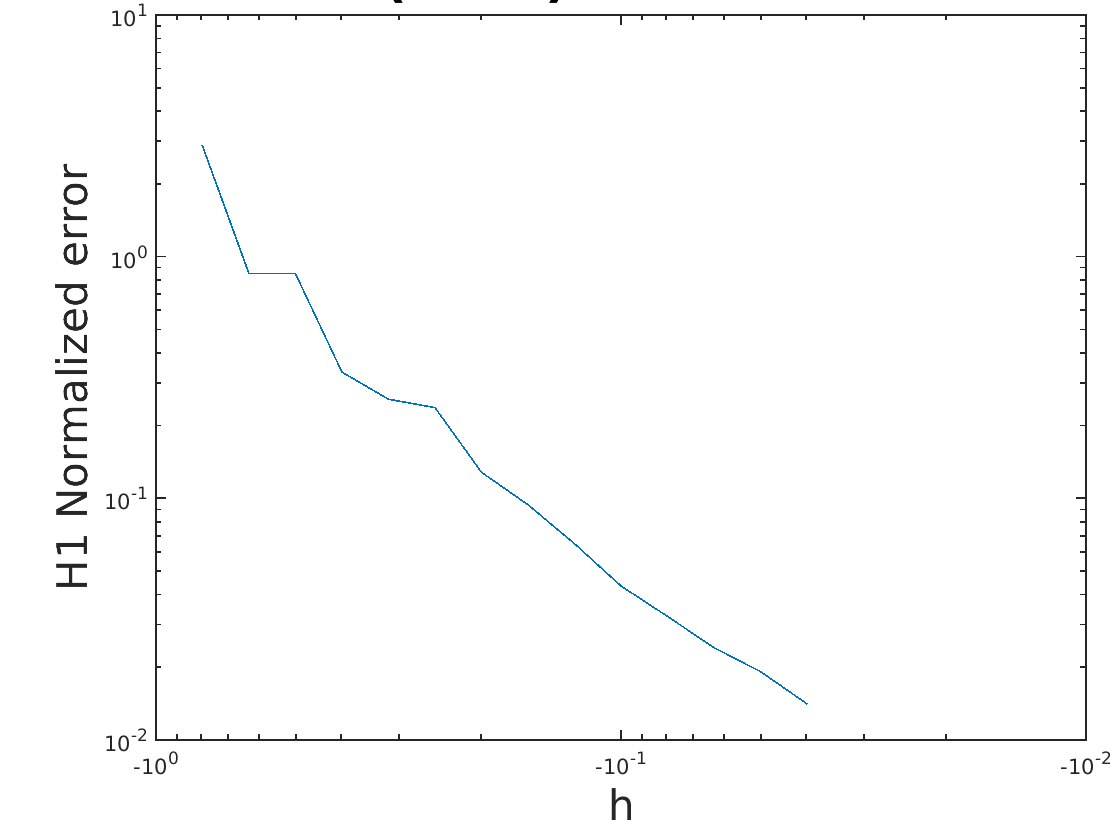
\includegraphics[width=.48\textwidth]{periodique/H1_Acst} \\
  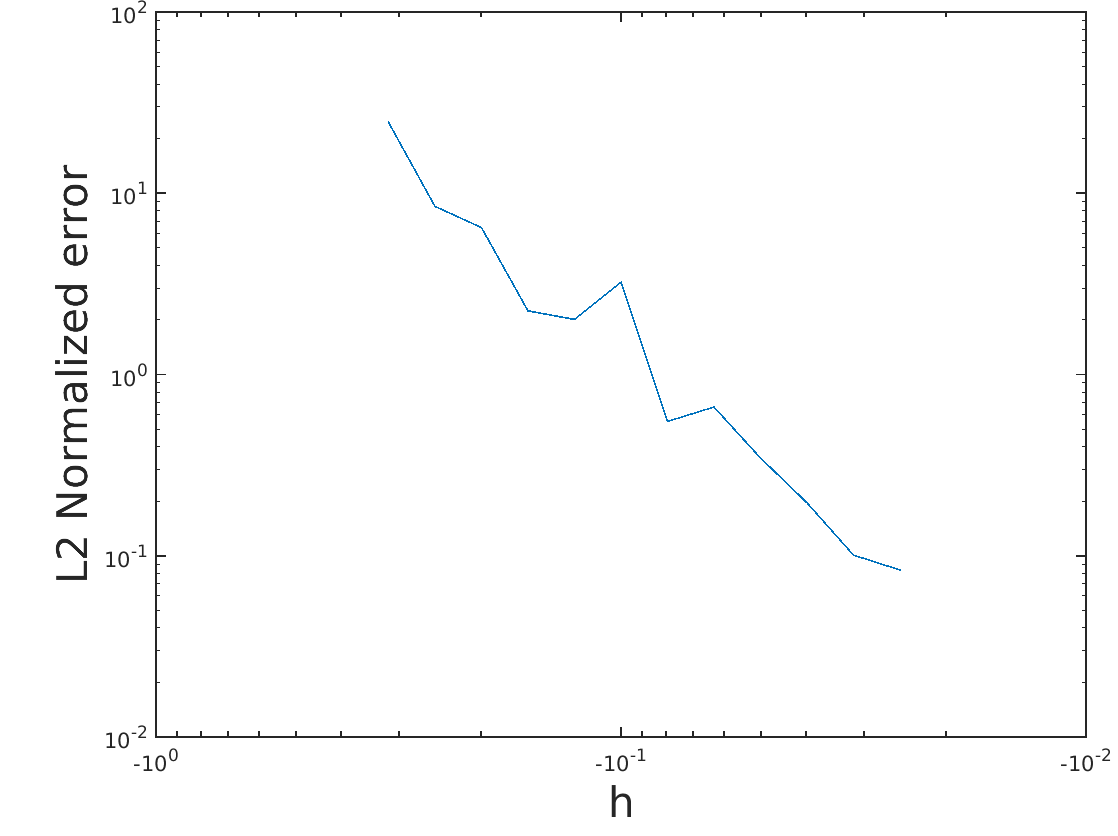
\includegraphics[width=.48\textwidth]{periodique/L2_Avar} 
  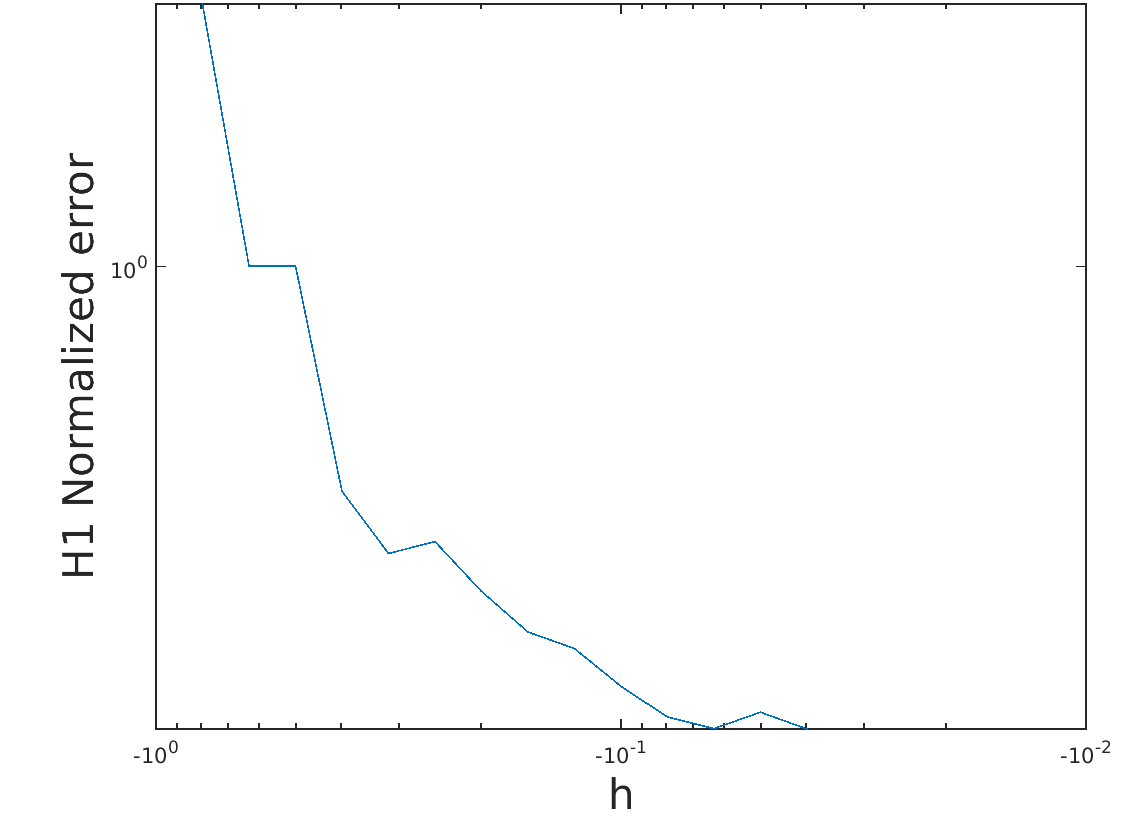
\includegraphics[width=.48\textwidth]{periodique/H1_Avar}
  \caption{Erreur normalisée pour la norme L2 et erreur normalisée pour la norme H1 dans le cas A variable.}
  \label{fig:avar}
\end{figure}

\end{document}

%%% Local Variables:
%%% mode: latex
%%% TeX-master: t
%%% End:
